\section{Resoconto delle attività di verifica}
In questa sezione vengono descritti ed analizzati gli esiti delle attività di verifica su tutti i documenti destinati alla consegna.

\subsection{Revisione dei requisiti}

\subsubsection{Analisi statica dei documenti}
I membri del gruppo \Gruppo{} hanno analizzato i documenti mediante la tecnica di walkthrough che ha portato all'individuazione di 
alcuni errori ortografici e grammaticali, grazie anche agli strumenti di controllo ortografico integrati negli editor per la produzione
della documentazione che il gruppo ha deciso di utilizzare.

\subsubsection{Esiti verifiche automatizzate}
Attualmente, l'unico valore che può essere calcolato per \glo{verificare} se la garanzia di qualità che il gruppo ritiene fornire è
soddisfatta, è data dall'Indice di Gulpease (MPC6).
%Per poter calcolare questo indice, viene utilizzato come strumento il "Calcolatore dell'Indice Gulpease" ospitato a \href{https://farfalla-project.org/readability_static/}{questo indirizzo}.
%Non vengono contati per l'indice di Gulpease il testo presente nelle seguenti parti o sezioni del documento:
%\begin{itemize}
  %  \item Indice;
  %  \item Registro delle modifiche;
  %  \item Riferimenti.
%\end{itemize}
Nella seguente tabella sono riportati i risultati degli indici di Gulpease ottenuti dai documenti per ogni periodo, successivamente ci sarà un grafico che riporterà l'andamento degli indici di Gulpease per ogni documento a seconda del periodo.

\paragraph{Legenda}
\begin{itemize}
	\item \textbf{Documento}: Nome del documento;
	\item \textbf{RR}: Periodo di revisione dei requisiti;
	\item \textbf{RP}: Periodo di revisione di progettazione;
	\item \textbf{RQ}: Periodo di revisione di qualifica;
	\item \textbf{RA}: Periodo di revisione di accettazione;
	\item \textbf{-}: Valore inesistente;
	\item  \textbf{Colore giallo}: Indica che il valore ottenuto è accettabile;
	\item  \textbf{Colore verde}: Indica che il valore ottenuto è ottimo. 
\end{itemize}
\newpage
{
\rowcolors{2}{grigetto}{white}
\renewcommand{\arraystretch}{1.5}
\centering
\begin{longtable}{C{4cm} C{1cm} C{1cm} C{1cm} C{1cm}}
\caption{Elenco dei indici di Gulpease }\\
\rowcolor{darkblue}
\textcolor{white}{\textbf{Documento}} & \textcolor{white}{\textbf{RR}} &
\textcolor{white}{\textbf{RP}} & \textcolor{white}{\textbf{RQ}} & 
\textcolor{white}{\textbf{RA}} \\
\hline
\endhead
\AdRv{1.0.0} & \textcolor{verde}{\textbf{95}} & - & - & -\\
\PdPv{1.0.0} & \textcolor{verde}{\textbf{100}} & - & - & -\\
\PdQv{1.0.0} & \textcolor{verde}{\textbf{100}} & - & - & - \\

\NdPv{1.0.0} & \textcolor{giallo}{\textbf{75}} & - & - & -\\
\SdFv{1.0.0} & \textcolor{verde}{\textbf{94}} & - & - & -\\

\Glossariov{1.0.0} & \textcolor{giallo}{\textbf{67}} & - & - & -\\

VI\_2019\_12\_18 & \textcolor{verde}{\textbf{100}} & - & - & -\\
VE\_2019\_12\_16 & \textcolor{giallo}{\textbf{65}} & - & - & -\\
VI\_2019\_12\_13 & \textcolor{verde}{\textbf{92}} & - & - & -\\
VI\_2019\_12\_10 & \textcolor{verde}{\textbf{100}} & - & - & -\\
VI\_2019\_12\_06 & \textcolor{verde}{\textbf{83}} & - & - & -\\
VI\_2019\_12\_03 & \textcolor{verde}{\textbf{83}} & - & - & -\\
VI\_2019\_11\_27 & \textcolor{verde}{\textbf{100}} & - & - & -\\
VI\_2019\_11\_20 & \textcolor{verde}{\textbf{87}} & - & - & -\\

\end{longtable}

%\begin{figure}[h]
%	\centering
%	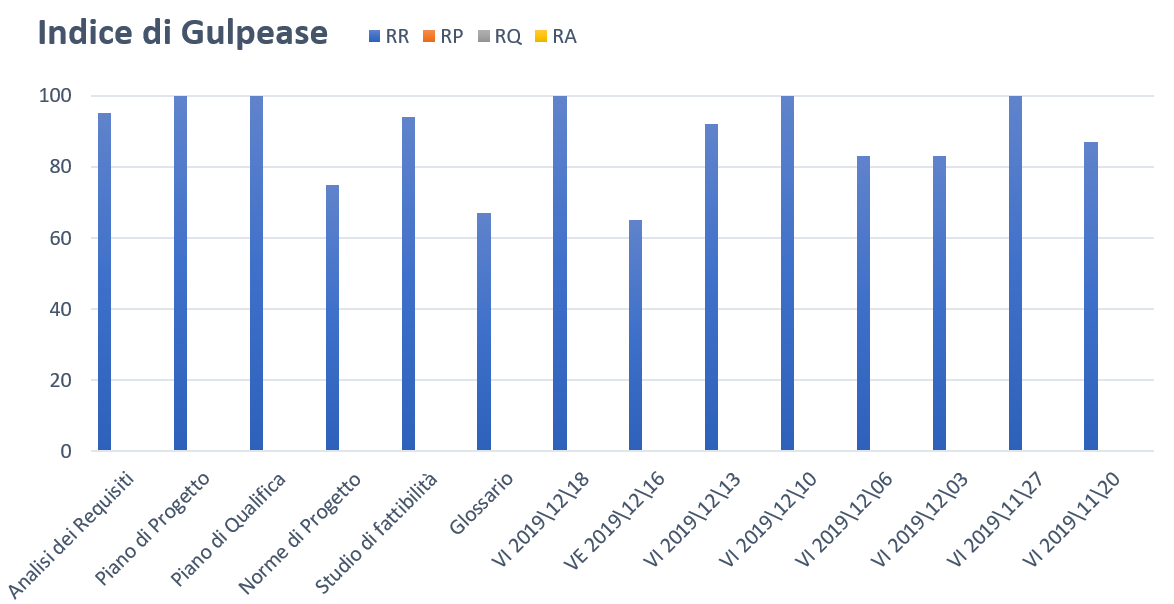
\includegraphics[scale=0.50]{Sezioni/Immagini/IG-Grafico.png}
%	\caption{Grafico andamento dell'Indice di Gulpease per ogni periodo e documento}
%\end{figure}
%}

	\pgfplotsset{width=17cm, height=8.5cm}
	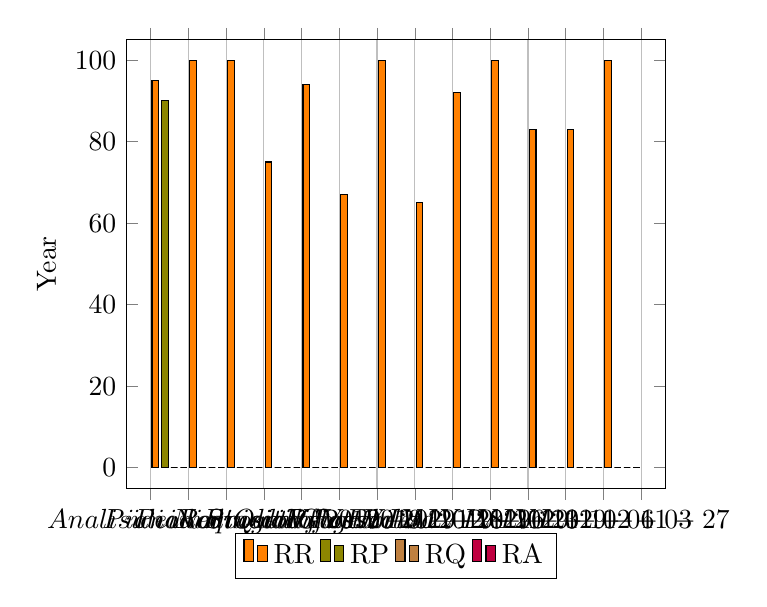
\begin{tikzpicture}
	\begin{axis}[
	x tick label style={
		/pgf/number format/1000 sep=},
	ylabel=Year,
	enlargelimits=0.05,
	legend style={at={(0.5,-0.1)},
		anchor=north,legend columns=-1},
	ybar interval=0.7,
symbolic x coords={$Analisi dei Requisiti$, $Piano di Progetto$, $Piano di Qualifica$, $Norme di Progetto$, $Studio di fattibilita$, $Glossario$,
$VI 2019-12-18$, $VE 2019-12-16$, $VI 2019-12-13$, $VI 2019-12-10$, $VI 2019-12-06$, $VI 2019-12-03$, $VI 2019-11-27$, $VI 2019-11-20$},
xtick=data
]
\addplot[fill=orange] coordinates
{($Analisi dei Requisiti$, 95) ($Piano di Progetto$, 100) ($Piano di Qualifica$, 100) 
	($Norme di Progetto$, 75) ($Studio di fattibilita$, 94) ($Glossario$, 67)
	($VI 2019-12-18$, 100) ($VE 2019-12-16$, 65) ($VI 2019-12-13$, 92) ($VI 2019-12-10$, 100) 
	($VI 2019-12-06$, 83) ($VI 2019-12-03$, 83) ($VI 2019-11-27$, 100) ($VI 2019-11-20$, 87)};

\addplot [fill=olive] coordinates
{($Analisi dei Requisiti$, 90) ($Piano di Progetto$, 0) ($Piano di Qualifica$, 0) 
	($Norme di Progetto$, 0) ($Studio di fattibilita$, 0) ($Glossario$, 0)
	($VI 2019-12-18$, 0) ($VE 2019-12-16$, 0) ($VI 2019-12-13$, 0) ($VI 2019-12-10$, 0) 
	($VI 2019-12-06$, 0) ($VI 2019-12-03$, 0) ($VI 2019-11-27$, 0) ($VI 2019-11-20$, 0)};

\addplot [fill=brown] coordinates
{($Analisi dei Requisiti$, 0) ($Piano di Progetto$, 0) ($Piano di Qualifica$, 0) 
	($Norme di Progetto$, 0) ($Studio di fattibilita$, 0) ($Glossario$, 0) 
($VI 2019-12-18$, 0) ($VE 2019-12-16$, 0) ($VI 2019-12-13$, 0) ($VI 2019-12-10$, 0) 
($VI 2019-12-06$, 0) ($VI 2019-12-03$, 0) ($VI 2019-11-27$, 0) ($VI 2019-11-20$, 0)};
\addplot [fill=purple] coordinates
{($Analisi dei Requisiti$, 0) ($Piano di Progetto$, 0) ($Piano di Qualifica$, 0) 
	($Norme di Progetto$, 0) ($Studio di fattibilita$, 0) ($Glossario$, 0)
	($VI 2019-12-18$, 0) ($VE 2019-12-16$, 0) ($VI 2019-12-13$, 0) ($VI 2019-12-10$, 0) 
	($VI 2019-12-06$, 0) ($VI 2019-12-03$, 0) ($VI 2019-11-27$, 0) ($VI 2019-11-20$, 0)};

\legend{
	RR,
	RP,
	RQ,
	RA
}
\end{axis}
\end{tikzpicture}